%
%
%
%
%
%
%
%
%
%
%
%
%
%
%
%
%
%
%
%
%
%
%
%
%
%
%
%
%
%
%
%
%
%
%
%
%
%
%
%
%
%
%
%
%
%
%
%
%
%
%
%
%
%
%
%
%
%
%
%
%
%
%
%
%
%
%
%
%
%
%
%
%
%
%
%
%
%
%
%
%
%
\begin{document}\renewcommand{\theenumi}{(\roman{enumi})}%


\maketitle

\begin{abstract}
Nonparametric estimation of the conditional distribution of a response given high-dimensional features is a challenging problem.  In many settings it is important to allow not only the mean but also the variance and shape of the response density to change flexibly with features, which are massive-dimensional with a distribution concentrated near a lower-dimensional subspace or manifold.  We propose a  multiscale model based on a novel stick-breaking prior placed on the dictionary weights.  The algorithm scales efficiently to massive numbers of features, and can be implemented efficiently with slice sampling.  State of the art predictive performance is demonstrated for toy examples and a real data application.
\end{abstract}

% \tableofcontents

\section{Introduction}


% opening
Massive datasets are becoming a ubiquitous by-product of modern scientific and industrial applications. These data present statistical and computational challenges for machine learning because many previously developed approaches do not scale-up sufficiently.  Specifically, challenges arise because of the ultrahigh-dimensionality, and relatively low sample size (the ``large p, small n'' problem).  Parsimonious models for such big data assume that the density in the ambient dimension concentrates around a lower-dimensional (possibly nonlinear) subspace.  Indeed, a plethora of methodologies are emerging to estimate such lower-dimensional ``manifolds'' from high-dimensional data \cite{Manifold, Maggioni}.  

We are interested in using such lower-dimensional embeddings to obtain estimates of the conditional distribution of some target variable(s).  This \emph{conditional regression} setting arises in a number of important application areas, including neuroscience, genetics, and video processing.  For example, one might desire automated estimation of a predictive density for a continuous neurologic {\em phenotype} of interest, such as intelligence or a creativity score, on the basis of available data for a patient including neuroimaging.  The challenge is to estimate the probability density function of the phenotype {\em nonparametrically} based on an $\mathcal{O}(10^6)$ dimensional image of the subject's brain.  It is crucial to avoid parametric assumptions on the density, such as Gaussianity, while allowing the density to change flexibly with predictors.  Otherwise, one can obtain misleading predictions and poorly characterize predictive uncertainty.

There is a rich machine learning and statistical literature on conditional density estimation of a response $y \in \mathcal{Y}$ given a set of features (predictors) $x=(x_1, x_2, \ldots, x_p)\in \mathcal{X}$. Common approaches include hierarchical mixtures of experts \cite{mixtureexperts,jiang1999}, kernel methods \cite{fan1996,fanyim2004,holmes2010,fu2011}, Bayesian finite mixture models \cite{nott2012,tran2012,norets2012} and Bayesian nonparametrics 
\cite{griffin06, dunson2007, DunsonPark, chung2009, tokdar2010}.  

% challenge
However, there has been limited consideration of scaling to large $p$ settings, with the variational Bayes approach of \cite{tran2012} being a notable exception. For dimensionality reduction, Tran et al. follow a greedy variable selection algorithm.  Their approach does not scale to the sized applications we are interested in. For example, in a problem with $p=1,000$ and $n=500$, they reported a CPU time of 51.7 minutes for a single analysis.  We are interested in problems with  $p$ having many more orders of magnitude, requiring a faster computing time while also accommodating flexible non-linear dimensionality reduction (variable selection is a limited sort of dimension reduction).  To our knowledge, there are no nonparametric density regression competitors to our approach, which maintain a characterization of uncertainty in estimating the conditional densities; rather, all sufficiently scalable algorithms provide point predictions and/or rely on restrictive assumptions such as linearity.  

In big data problems, scaling is often accomplished using divide-and-conquer techniques. Well known examples are classification and regression trees (CART) \cite{CART} and multivariate adaptive regression splines (MARS) \cite{MARS}. These algorithms fit surfaces to data by explicitly dividing the input space into a nested sequence of regions, and by fitting simple surfaces  within these regions. Though these methods are appealing in providing a simple, flexible and interpretable mechanism of dimension reduction, it is well known that single tree estimates commonly have high variance and poor performance.  There is a rich literature proposing improvements based on bagging \cite{Bagging}, boosting \cite{Boosting} and random forests \cite{RandomForest}. Though these algorithms can substantially improve mean square error performance, computation can be expensive and performance degrades as dimensionality $p$ increases.

In fact, a significant downside of many divide-and-conquer algorithms is their poor scalability to high dimensional predictors. As the number of features increases, the problem of finding the best splitting attribute becomes intractable so that CART, MARS and multiple trees models cannot be efficiently applied. Also mixture of experts models become computationally demanding, since both mixture weights and dictionary densities are predictor dependent. In an attempt to make mixtures of experts more efficient, sparse extensions relying on different variable selection algorithms have been proposed \cite{SparseMoF}. However, performing variable selection in high dimensions is effectively intractable: algorithms need to efficiently search for the best subsets of predictors to include in weight and mean functions within a mixture model, an NP-hard problem.

% approach
 In order to efficiently deal with massive datasets, we propose a novel multiscale approach which starts by learning a multiscale dictionary of densities,. This tree is efficiently learned in a first stage using a fast and scalable graph partitioning algorithm applied to the high-dimensional observations \cite{metis}.  Expressing the conditional densities $f(y|x)$ for each $x \in \mathcal{X}$ as a convex combination of coarse-to-fine scale dictionary densities, the learning problem in the second stage estimates the corresponding multiscale probability tree.  This is accomplished in a Bayesian manner using a novel multiscale stick-breaking process, which allows the data to inform about the optimal bias-variance tradeoff; weighting coarse scale dictionary densities more highly decreases variance while adding to bias if the finer scale structure is needed.  This results in a model that allows borrowing information across different resolution levels and reaches a good compromise in terms of the bias-variance tradeoff. We show that the algorithm scales efficiently to massive numbers of features. 


\section{Setting} \label{section:setting}
Let $X \from \Omega \to \mc{X} \subseteq \Real^p$ be a 
$p$-dimensional Euclidean vector-valued predictor random variable, taking values $x \in \mc{X}$, with a marginal probability distribution $F_X$.  
Similarly, let $Y \from \Omega \to \mc{Y}$ 
% $ \subseteq \Real^q$ be a $p$-dimensional Euclidean vector
be a $\mc{Y}$-valued target random variable, taking values $y \in \mc{Y}$, with a marginal probability distribution $F_Y$ (we will specify specific forms of $\mc{Y}$, e.g., $\mc{Y} \subseteq \Real^q$, below).  We assume that the pair $(X,Y)$ is sampled from a joint distribution, $F_{X,Y} \in \mc{F}$.

For inferential expedience, we  posit the existence of  a latent random variable $\mb{\eta} \from \Omega \to \mc{M} \subseteq \mc{X}$, where $\mc{M}$ is only $d$ ``dimensional'' and $d \ll p$.   
% $mb{mu} \from \Omega \to \mc{M} \subseteq \Real^d$, a latent $d \ll p$-dimensional vector-valued random variable. 
Note that $\mc{M}$ need not be a linear subspace of $\mc{X}$, rather, $\mc{M}$ could be, for example,  a union or affine subspaces, or a smooth compact Riemannian manifold.  Regardless of the nature of $\mc{M}$, we assume that we can approximately decompose the joint distribution as follows,  $F_{X,Y,\mb{\eta}}=F_{X,Y|\mb{\eta}}F_{\mb{\eta}} = F_{Y|X, \mb{\eta}} F_{X | \mb{\eta}} F_{\mb{\eta}} \approx F_{X|\mb{\eta}} F_{Y|\mb{\eta}} F_{\mb{\eta}}$.  In  words, we assume that the \emph{signal} approximately concentrates around a low-dimensional latent space, $F_{Y|X,\mb{\eta}}=F_{Y|\mb{\eta}}$.  Note that this is a much less restrictive assumption than the commonplace assumption in manifold learning that the marginal distribution $F_X$ concentrates around a low-dimensional latent space.  %Moreover, these assumptions we make for inferential convenience, rather than a belief that the true signal concentrates around a low-dimensional anything. On the contrary, the truth, we believe, is much more complex and beautiful than anything we could ever hope to write down formally!


% Let $y \in  \mathcal{Y} \subseteq \Real$ be a real-valued target variable. We further assume that the conditional distribution is a function of only the position $\eta$ of $x$ within the subspace $\mathcal{M}$, $f(y|x)=f(y|\eta)$. Let $x$ and $y$ be sampled from some true but unknown joint distribution. We would like to learn $f(y| x)$.  We assume that we obtain $n$ independently and identically sampled observations, $(x_i,y_i) $, for $i \in \{1,2,\ldots,n\}$.  Our proposed model introduced in \S \ref{section:model} is very general in accommodating an unknown density $f(y|x)$ which changes according to the location of $x$ in the lower-dimensional subspace.  However, for exposition and testing of the model, it is useful to consider a simple example in which $x$ lives on a smooth one-dimensional Riemannian submanifold embedded in $\Real^p$, and  $y$ is a univariate Gaussian random variable whose mean and variance vary with the location of $x$ along its geodesic.  

To provide some intuition around this model, we provide the following concrete example where the distribution of $Y$ is a Gaussian function of the coordinate $\eta$ along the swissroll, which is embedded in a high-dimensional ambient space:
\begin{subequations} \label{eq:linear}
\begin{align}
	Y | \eta &\sim \mc{N}(\mu(\eta) ,\sigma(\eta)) \\
X_r &\sim \mc{N}(0,1) \text{ for } r \in \{3, \ldots, p\}, \qquad 	X_1 = \eta \sin (\eta), \qquad X_2 = \eta \cos (\eta) \\
	% X_r | \eta &=  \mc{N}(\mu_r,\sigma_r), \\
	\eta  &\sim U(0,1), 
\end{align}
\end{subequations}
% where $(\mu_1,\sigma_1)=(\eta \sin (\eta),0)$, $\mu_2=\eta \cos(\eta)$, $\mu_r=0$ for $r = \{3,\ldots,p\}$ and
% .
% Let $\mb{\eta}$ be distributed according to a uniform distribution on (0,1), $\mb{\eta} \sim U(0,1)$. Let $F_X$ be constructed as follows: $x_1=\eta \sin (\eta)$, $x_2=\eta \cos (\eta)$, and $X_j \sim \mc{N}(0,1)$ for all $j \in \{3, \ldots, p\}$.  Moreover, let $Y \sim \mc{N}(\mb{\eta},\mb{\eta}+1)$.  Thus, c
where $\mc{N}(\mu,\sigma)$ denotes a Gaussian distribution with mean $\mu$ and standard deviation $\sigma$, and $U(0,1)$ denotes the uniform distribution on $(0,1)$.
Clearly, $Y$ is conditionally dependent on $\mb{\eta}$, which is the low-dimensional signal manifold, of which $X$ is also a function.  In particular, $X$ lives on a swissroll embedded in a $p$-dimensional ambient space, but $Y$ is only a function of where $\mb{\eta}$ is along the swissroll. The left panels of Figure \ref{fig:swiss} depict this concrete example when $\mu(\eta)=\eta$ and $\sigma(\eta)=\eta + 1$.


\begin{figure}[htbp]
	\centering
		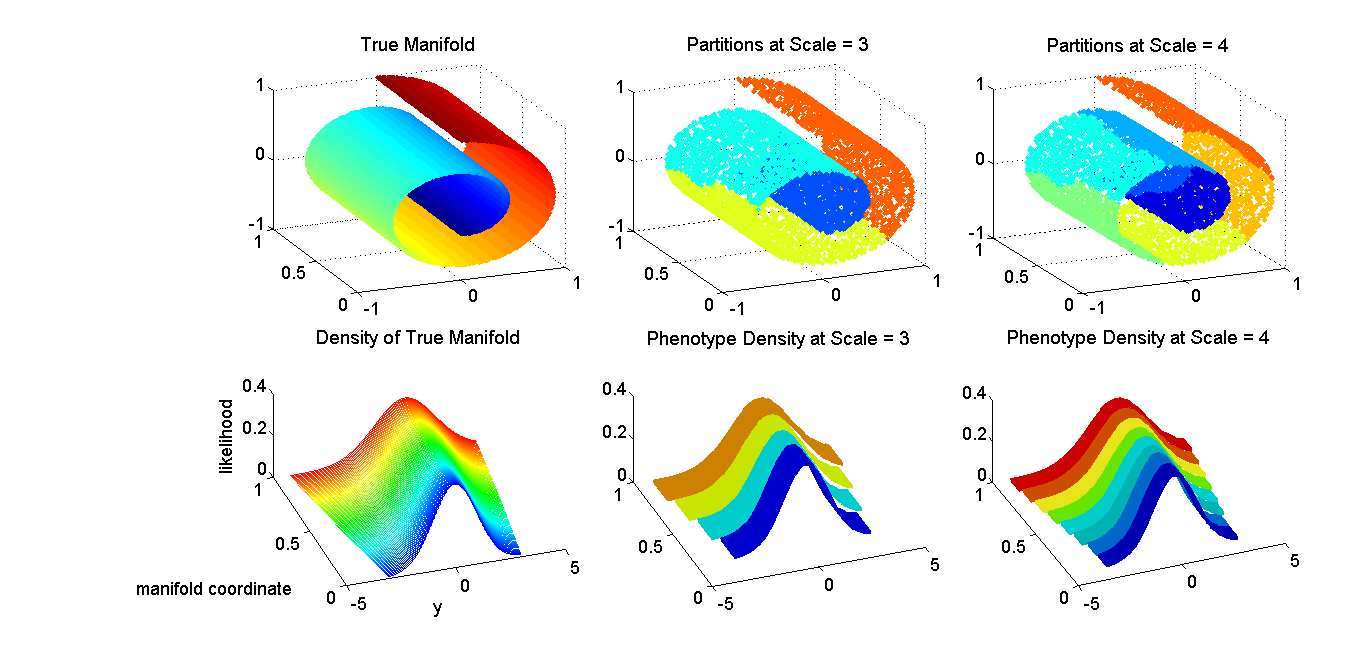
\includegraphics[width=1\linewidth]{../figs/density3D(FF4)}
	\caption{Illustration of our generative model and algorithm on a swissroll. The top left panel shows the manifold $\mc{M}$ (a swissroll) embedded in a $p$-dimensional ambient space, where the color indicates the coordinate along the manifold, $\eta$ (only the first 3 dimensions are shown for visualization purposes). The bottom left panel shows the distribution of $Y$ as a function of $\eta$, in particular, $F_{Y|\eta}=\mc{N}(\mb{\eta},\mb{\eta}+1)$. The middel and right panels show our estimates of $F_{Y|\mb{\eta}}$ at scales 3 and 4, respectively, which follow from partitioning our data.}
	\label{fig:swiss}
\end{figure}


\section{Goal} \label{sec:goal}

Our goal is to develop an approach to learn about $F_{Y|X}$ from $n$ pairs of observations that we assume are sampled exchangeable from the joint distribution, $(x_i,y_i) \sim F_{X,Y} \in \mc{F}$. Let $\mc{D}^n=\{(x_i,y_i)\}_{i \in [n]}$, where $[n]=\{1,\ldots, n\}$.  More specifically, we seek to obtain a posterior over $F_{Y|X}$.  We insist that our approach satisfies several desiderata, including most importantly: (i) scales up to $p \approx 10^6$ in reasonable time,  (ii) yields good empirical results, and (iii) automatically adapts to the complexity of the data corpus.  To our knowledge, no extant approach for estimating conditional densities or posteriors thereof satisfies even our first criterion. Below, we provide a general multiscale approach to this problem (\S \ref{sec:method}), followed by our specific choices (\S \ref{sub:spec}), results on simulated (\S \ref{sec:sim}) and real neuroscience (connectomics) data (\S \ref{sub:real}), and a discussion (\S \ref{sec:disc}).

% 
% 
% Let $g_n \from \mc{D}^n \to \mc{F}$ denote an estimator of the conditional distribution from data, and let $\mh{F}$ denote its corresponding estimate.  Let $g=g_1, g_2, \ldots$ indicate a sequence of said estimators, which we refer to as a \emph{rule}.  Let $g^*$ and $\mh{F}^*$ indicate a universally consistent estimator and estimate, respectively:
% 
% \begin{align}
% g^* = \{\mh{F}_n := g_n(\mc{D}^n) \overset{n,p \conv \infty}{\longrightarrow} F_{X,Y} \, \forall \, F_{X,Y} \in \mc{F} \text{ as }  p/n \conv c \geq 0\}
% \end{align}



\section{Methodology} \label{sec:method}

\subsection{\msd~Framework}

We propose here a general modular approach which we refer to as \uline{m}ulti\uline{s}cale \uline{d}ictionary learning for \uline{e}stimating conditional \uline{d}istribution\uline{s} (``\msd''). \msd~consists of three components: (i) a tree decomposition of the space, (ii) an embedding of the data into a lower-dimensional space, %$\psi \from (\mc{X},\mc{Y}) \to \Xi$ taking values $(\xi_x,\xi_y) \in (\Xi_x,\Xi_y) :=\Xi $,
 and (iii) an assumed form of the conditional probability model. %, $\mc{P}_{\xi_y|\xi_x}$. 
% There are many choices that one could make for each of the three components, we describe  that we organize into three types, we could (a) choose functions, (b) estimate functions


\paragraph{Tree Decomposition}
A tree decomposition $\tau$ yields a multiscale partition of the data or the ambient space in which the data live.
Let $(\mc{W},\rho_W, F_W)$ be a measurable metric space, where $F_W$ is a Borel probability measure, $\mc{W}$, and $\rho_W \from \mc{W} \times \mc{W} \to \Real$ is a metric on $\mc{W}$.  Let $B_r^{\mc{W}}(w)$ be the $\rho_W$-ball inside $\mc{W}$ of radius $r > 0$ centered at $w \in \mc{W}$. For example, $\mc{W}$ could be the data corpus $\mc{D}_n$, or it could be $\mc{X} \times \mc{Y}$. We define a tree decomposition as in \cite{Allard2012,ChenMaggioni12}.  A partition tree $\tau$ of $\mc{W}$ consists of a collection of cells, $\tau=\{C_{j,k}\}_{j \in \ZZ, k \in \mc{K}_j}$.  At each scale $j$, the set of cells $C_j=\{C_{j,k}\}_{k \in \mc{K}_j}$ provides a disjoint partition of $\mc{W}$ almost everywhere, and $\mc{K}_j$ is the set of partitions at scale $j$.  We define $j=0$ as the root node/cell.  For each $j > 0$,  each $C_{j,k}$ has a unique parent node $C_{j-1,k'}$ containing $C_{j,k}$, and conversely, any $C_{j,k} \subseteq C_{j-1,k'}$ is called a child of $C_{j-1,k'}$.


% \begin{definition}\label{Def:tree} A \emph{tree decomposition} $\tau \in \Lambda$ of a $d'$-dimensional metric measure space $(\mc{W}, \rho_W, F_W)$ is a collection of open sets $\{C_{j,k}\}_{j \in \mathcal{K}_k,k \in \ZZ}$, called \emph{cells}, satisfying:
% \begin{enumerate}\itemsep0pt
% 	\item for all $j \in \ZZ$, $F_W(\mc{W} \backslash \cup_{k \in \mc{K}_j} C_{j,k} )=0$,
% 	\item for all $j' \geq j$ and $k' \in \mc{K}_j$, either $C_{j',k'} \subseteq C_{j,k}$ or $F_W(C_{j',k} \cap C_{j,k})=0$,
% 	\item for $j < j'$ and $k' \in \mc{K}_{j'}$, there exists a unique $k \in \mc{K}_j$ such that $C_{j',k'} \subseteq C_{j,k}$,
% 	\item each $C_{j,k}$ contains a point $c_{j,k}$ such that $B_{r \cdot \theta^{j}}^{\mc{W}}(c_{j,k}) \subseteq C_{j,k} \subseteq B_{\theta^{j}}^{\mc{W}}(c_{j,k})$ for a constant $r$ depending on the intrinsic geometric properties of $\mc{W}$.  In particular, we have $F_{{j,k}} \approx \theta^{d'j}$, for any $0 < \theta < 1$.
% \end{enumerate}
% \end{definition}
% The first condition means that at each scale, the set of cells covers the space almost everywhere. The second and third condition together mean that as we descend the tree, going from a coarser to finer scale, for a given cell at scale $j$, it is the child of a single coarser scale cell, such that its intersection with any other coarser scale cell has measure zero. The fourth condition means that there exists a point $c_{j,k}$ which is effectively the location of cell $C_{j,k}$, in that it is in $C_{j,k}$, and that all other points in $C_{j,k}$ are within a small distance of $c_{j,k}$.  

Let $A_{j,k}=\{k' \in \mc{K}_{j'} : j' < j$ s.t. $C_{j,k} \subseteq C_{j',k'}\}$ denote the ancestors of $C_{j,k}$, and let $D_{j,k}=\{k' \in \mc{K}_{j'} : j' > j$ s.t. $C_{j',k'} \subseteq C_{j,k}\}$ denote the descendants of $C_{j,k}$.
% Let $P_{j,k}$ be the path of $C_{j,k}$, that is, $P_{j,k}=\{C_{j',k'} : j' < j, C_{j',k'} \supseteq C_{j,k}\}$ be the \emph{path} along the tree for point $w \in \mc{W}$. 
% Given a tree decomposition, we can approximate $F_{Y|X}$ at each scale $j$ by $\cup_{k \in \mc{K}_j} F_{Y|C_{j,k}}$.  
Figure \ref{graph}(i) depicts a binary tree decomposition for some data (note that the tree need not be binary).

\begin{figure}[h] 

\setlength{\unitlength}{2mm}
\begin{picture}(30, 26)

 \put(9, 22){\bfoo(i)\efoo}
 
 \put(20, 22){$\mathcal{\mc{W}}_{11} = \mathcal{\mc{W}}$}
\put(20, 20){\vector(-1, -1){3}}
\put(20, 20){\vector(1, -1){3}}

 \put(14, 14){$\mathcal{\mc{W}}_{21}$}
 \put(23, 14){$\mathcal{\mc{W}}_{22}$}
 
\put(14, 12){\vector(-1, -1){3}}
\put(14, 12){\vector(1, -1){3}}

\put(25, 12){\vector(-1, -1){3}}
\put(25, 12){\vector(1, -1){3}}

 \put(9, 6){$\mathcal{\mc{W}}_{31}$}
 \put(16, 6){$\mathcal{\mc{W}}_{32}$}
 
 \put(20,6){$\mathcal{\mc{W}}_{33}$}
 \put(28, 6){$\mathcal{\mc{W}}_{34}$}
  
  \put(13, 3){$\ldots$}
  \put(25, 3){$\ldots$}

% -- square
\put(6, 25){\line(1, 0){56}}
\put(6, 25){\line(0, -1){27}}
\put(6, -2){\line(1, 0){56}}
\put(62, 25){\line(0, -1){27}}

%% right graph

\put(36, 14){$w_i \in \mc{W}$}
\put(39, 13){\line(0, -1){1}}
\put(39, 12){\vector(1, 0){5}}

\put(37, 22){\bfoo(ii)\efoo}
  \put(48, 22){$\mc{W}_{11}$}
\put(48, 20){\vector(-1, -1){3}}
\put(48, 20){\vector(1, -1){3}}

 \put(51, 14){$\mc{W}_{22}$}
 \put(53, 12){\vector(-1, -1){3}}
\put(53, 12){\vector(1, -1){3}}

 \put(48,6){$\mc{W}_{33}$}
  \put(53, 3){$\ldots$}
  \put(18, -0.5){\bfoo(iii)\efoo}
 \put(22, -0.5){$f(y_i|x_i)=p_{11}f_{11}+p_{22}f_{22}+p_{33}f_{33}+ \ldots$}

\end{picture} \caption{(i) Multiscale partition of the data. (ii) Path through the tree for $x_i \in \Real^p$. (iii) Conditional density of $y_i$ given $x_i$ defined as a convex combination of densities along the path.}\label{graph}
\end{figure}

\paragraph{Embeddings}
At each scale, for each cell, we consider some embedding $\psi_{j,k} \from C_{j,k} \to \Xi$, where $(\xi_x,\xi_y) \in \Xi$.  Thus, we can approximate $F_{Y|X}$ at scale $j$ by $\cup_{k \in \mc{K}_j} F_{\mb{\xi}_y| \mb{\xi}_x}$.   
% While we could estimate $\psi$'s from the data, for example, as in  \cite{Allard2012}, we chose instead to assume that $\psi_{j,k}((x,y))=\delta(x: x \in \mc{C}_{j,k})$, where .  We chose to simply assume $\psi$
 % chose $\psi$ to be a linear projection of the data onto the best fitting $d$-dimensional hyperplane.  %In general, one can either choose or learn these embeddings.

\paragraph{Family} Each $F_{\mb{\xi}_y | \mb{\xi}_x}$ is an element of a family of distributions, $\mc{F}_{\cdot | \cdot}$.  This family might be quite general, e.g., all possible conditional densities, or quite simple, e.g., Gaussian distributions.

% \paragraph{Prior} We further assume a prior, $\pi=\{\pi_{j,k}\}_{j \in \mc{K}_j, j \in \ZZ}$ over all paths of the tree. This prior facilitates finding an optimal bias/variance tradeoff, without having to choose a particular scale.

Thus, collectively, any multiscale Bayesian conditional density estimation procedure makes choices for the above three components.  This encompasses a wide range of possible approaches. 
% can be implemented using Pseudocode \ref{alg:ABCDE}.

% \begin{algorithm}
% 	\caption{ ``Ms. Deeds'' (MultiScale Dictionary learning for conditional DistributionS)} \label{alg:ABCDE}
% \begin{algorithmic}[1]
% 	\REQUIRE the data $\mc{D}^n$ and the following choices: (i) a partitioning scheme $\Lambda$, (ii) a class of embeddings $\Psi$, (iii) a family of potential conditional densities $\mc{F}$, (iv) a prior $\pi$ over scales
% 	\STATE Estimate a multiscale partition $\tau$ from the data $\mc{D}^n$ using $\Lambda$
% 	\STATE Estimate or choose embeddings $\psi_{j,k} \from C_{j,k} \to \ZZ$, where $\psi \in \Psi$ 
% 	\STATE Estimate $F_{Y|\psi_{j,k}(C_{j,k})}$ from the family $\mc{F}$
% 	\STATE Let $\mh{F}_{Y|X=x_i} = \sum_j \mh{F}_{Y | \psi_{j,k}(x_i) : x \in C_{j,k}}  \pi_{j,k}$ 
% 	\ENSURE $\mh{F}_{Y|X=x_i}$
% \end{algorithmic}
% \end{algorithm}

 % Consider  $$x_i \sim \mc{N}(\psi(\eta_i),\sigma^2 I),$$ where $\Psi =\{ \psi \from \mc{M} \to \Real^p\}$, $\eta_i \in \mc{M}$, $\sigma \in (0,\infty)$, $I$ is the $p\times p$ dimensional identity matrix.  Let $\mc{M}$ be a smooth compact Riemannian manifold, such as the swissroll or the S-manifold. For simplicity, let us assume that $\mc{M}$ is a curve. Let $\psi(\eta)= 1\eta$ with $1$ being a $p$-dimensional vector with all elements equal to $1$. Define the conditional $f(y|x)$ as a function of $\eta$, i.e. a mixture density with mixture weights depending on $\eta$.  We will show in \S \ref{section:simulation} that  our construction facilitates an estimate of the density of $y$.

\subsection{Specific Choices} \label{sub:spec}

% \begin{description}
	\paragraph{Tree Partition} Unlike classical harmonic theory which presupposes $\tau$ (e.g., in wavelets \cite{Daubechies1992}), we choose to learn $\tau$ from the data. Previously, Chen et al. \cite{ChenMaggioni12} developed a multiscale measure estimation strategy, and proved that there exists a scale $j$ such that the approximate measure is within some bound of the true measure, under certain relatively general assumptions.  We could, therefore, adopt that strategy for both $F_{X,Y}$ and $F_{X}$, and then divide to obtain $F_{Y|X}$.  Instead, we decided to simply partition the $X$'s, ignoring the $Y$'s in the partitioning strategy.  
	
	Our justification for this choice is as follows. First, sometimes there are many different $\mc{Y}$'s for many different applications.  In such cases, we do not want to bias the partitioning to any specific $\mc{Y}$'s, all the more so when new unknown $\mc{Y}$'s may later emerge.  Second, because the $X$'s are so much higher dimensional than the $Y$'s in our applications of interest, the partitions would be dominated by the $X$'s, unless we chose a partitioning strategy that emphasized the $Y$'s.  Thus, our strategy mitigates this difficulty (while certainly introducing others). 

	Given that we are going to partition using only the $X$'s, we still face the choice of precisely how to partition.  A fully Bayesian approach would construct a large number of partitions, and integrate over them to obtain our posteriors.  However, such a fully Bayesian strategy remains  computationally intractable at scale, so we adopt a hybrid strategy.  Specifically, we employ METIS \cite{METIS}, a well-known relatively efficient multiscale partitioning algorithm with demonstrably good empirical performance on a wide range of graphs.  Graph construction follows via computing all pairwise distances using $\rho_{uv}=\rho_W(w_u,w_v)=\norm{\mt{w}_u-\mt{w}_v}_2$, where $\mt{w}$ is the whitened $w$ (i.e., mean subtracted and variance normalized). We let there be an edge between $w_u$ and $w_v$ whenever  e$^{-\rho_{uv}^2} > t$, where $t$ is some threshold chosen to elicit the desired sparsity level.
	
	Applying METIS on the graph constructed in this way yields a single tree.  We then place a non-parametric prior $\pi$ over the leaves of the tree, to facilitate borrowing strength across the paths.  More specifically, we let $\pi$ be generated by a stick-breaking process \cite{stickbreaking}.  For each node $C_{j,k}$ in the partition tree, we define a stick length $V_{j,k} \sim \mbox{Beta}(1,\alpha)$.  The parameter $\alpha$ encodes the complexity of the model, with $\alpha=0$ corresponding to the case in which $f(y|x) = f(y)$. The stick-breaking process is defined as follows: 
	\begin{eqnarray*}
	\pi_{j,k}(x) \propto V_{j,k} \prod_{C_{j',k'} \in A_{j,k}} \left[1 - V_{j',k'}) \right],
	\end{eqnarray*}
	where  $\sum_{j=1}^k \pi_{j,k} = 1$.   We refer to this prior as a {\em multiscale stick-breaking process}. Note that this Bayesian nonparametric prior assigns a positive probability to all possible paths, including those not observed in the training data.  Thus, by adopting this Bayesian formulation, we are able to obtain posterior estimates for any newly observed data, regardless of the amount and variability of training data.  This is a pragmatically useful feature of the Bayesian formulation, in addition to the alleviation of the need to choose a scale \cite{ChenMaggioni12}.  %Moreover, by integrating over all paths, we are able to borrow information adaptively to the observed data.


\paragraph{Embedding} We let each $\psi_{j,k}$ simply be a Dirac delta function operating \emph{only on the $X$'s}.  This is because, in our application of interest, $X$'s are quite high-dimensional, and the $Y$'s are relatively low-dimensional (e.g., one-dimensional).  The choice of Dirac delta functions over, say, hyperplanes, alleviates the computational and theoretical difficulties of estimating hyperplanes via SVD and choosing the dimensions thereof. That said, both theoretical considerations imply that the relative computation cost to computing SVDs for each partition, versus partitioning, is  
% , rather, we assume $\psi_{j,k}(x)=1$ if an only if $x \in C_{j,k}$.  The Dirac function can result in significant computational savings versus linear embedding for each partition $C_{j,k}$.  In particular, the ratio of computational costs between partitioning and linear embedding is 
$\mc{O}(3^d/d^2)$, where $d$ is the intrinsic dimension \cite{Allard2012}. In practice, except for very low-dimensional intrinsic dimensional data, building the partition dominates \cite{Allard2012}.  Moreover, empirical results seem to be robust to choice of embedding dimension \cite{Lawlor2012}. Nonetheless, results from multiscale measure estimation \cite{ChenMaggioni12} suggest that choosing a Dirac delta function is sufficient to ensure accurate estimates of the empirical marginal measure, $F_X$, for some scale $j$.  Thus, we view our chosen strategy as the simplest approach, making code, computations, and theory all more tractable.  


\paragraph{Family} We let $\mc{P}=\mc{N}(\mb{m},\mb{\Sigma})$ be Gaussian for simplicity. Obviously, other choices, such as finite or infinite mixtures of Gaussians are also possible for continuous valued data.  Because we are interested in posteriors over the conditional distribution $F_{Y|X}$, we place relatively uninformative priors on $\mb{m}$ and $\mb{\Sigma}$, specifically, assuming the $y$'s have been whitened and are unidimensional,  
$m \sim \mc{N}(0,1)$ and $\sigma=\mc{IG}(a,b)$.




\subsection{Estimation}


% Parameters involved in the dictionary densities can be estimated using either frequentist or Bayesian methods. Bayesian methods are appealing since they can avoid singularities associated with traditional maximum likelihood inference, the prior has an appealing role as a regularizer, and we can characterize uncertainty in dictionary learning through the resulting posterior. Hence, parameters involved in dictionary densities will be estimated through Bayesian methods and inference on stick breaking weights and dictionary density parameters will be carried out using the Gibbs sampler. Details on full conditionals and Gibbs sampler steps can be found in the supplementary material.

%For this purpose, 
We introduce the latent variable $\ell_i \in \{1,\ldots,k\}$, for $i=1,\ldots,n$, denoting the multiscale level used by the $i^{th}$ observation.  
%Assuming data are normalized prior to analysis, we let $\eta_{j,k} \sim \mc{N}(0,1)$ and $\sigma_{j,k}=\mc{IG}(a,b)$ for the means and variances of the dictionary densities. 
Let $n_{j,k}$ be  the number of observations in $C_{j,k}$ . Each Gibbs sampler iteration can be summarized in the following steps:
% . Details on full conditionals and Gibbs sampler steps can be found in the supplementary material.
\dd{not clear to me that this is correct}

\begin{enumerate}
\item Update $\ell_i$ by sampling from the multinomial full conditional with 
\[\mbox{Pr}( \ell_i = j\, |\, \cdot) = \frac{ \pi_{j,k}(x_i)f_{j,k}(y_i|x_i) }{ \sum_{k'=1}^k \pi_{j,k'}(x_i)f_{j,k'}(y_i | x_i) } \label{eq:prS}\]

\item Update stick-breaking random variable $V_{j,k}(x_i)$, for $j=1, \ldots, |\mc{K}_j|$ and $i=1, \ldots, n$, from $\mbox{Beta}(\beta',\alpha')$ with $\beta'=1+n_{j,k}$ and $\alpha'=\alpha+\sum_{C_{j,K} \in D_{j,k}(x_i)} n_{j,k}(x_i)$.

\item Update $m_{j,k}(x_i)$ and $\sigma_{j,k}(x_i)$ by sampling from

\begin{align*}
	m_{j,k} \sim \mc{N}\left(\frac{\bar{y}_{j,k} n_{j,k}}{ \sigma_{j,k}} , (1+\frac{n_{j,k}}{\sigma_{j,k}})^{-1}\right), \quad
	 \sigma_{j,k} \sim \mc{IG}\bigg(a_{\sigma},b+0.5\sum_{i \in \mc{I}_{j,k}} \left(y_{i}-m_{j,k}\right)^2\bigg)	
\end{align*}

with $a_{\sigma}=a+n_{j,k}/2$, $\bar{y}_{j,k}$ being the average of the observation $\{y_i\}$ allocated to cell $C_{j,k}$ and $\mc{I}_{j,k}=\{i : \ell_i=j, x_i \in C_{j,k}\}$.

\end{enumerate}



\subsection{Predictions}\label{ch3:predictions}

Consider the case we want to predict the response $y_{n+1}$ for a future observation based on the predictors $x_{n+1}$. For each tree level, the new vector of predictors $x_n$ is allocated to subsets having closer centers with respect to $\rho_W$, acting as a Voronoi expansion. For a new observation the predictive density is defined as
\dd{what about all the other $x_i$'s? they must be in there.  also, where is $f\left(y_{n+1}|x_{n+1},\Omega\right)$ defined?  where is \ref{eq:base}? is this correct? }

\begin{equation*}
	p(y_{n+1}|x_{n+1}, y_1, \ldots, y_n) = \int f\left(y_{n+1}|x_{n+1},\Omega\right) dp\left(\Omega|y_1, \ldots, y_n\right) \label{predictive:MSB}
	\end{equation*}

with $f\left(y_{n+1}|x_{n+1},\Omega\right)$ defined as in (1) and $\Omega$ being the set of all parameters involved, i.e. weights, location and scale parameters. In order to make inference on the predictive density of $y_{n+1}$, at the $s$th  Gibbs sampler iteration, we will first sample parameters involved in \ref{eq:base} from its posterior, i.e. $\Omega^{(s)} \sim p\left(\Omega|y_1, \ldots, y_n\right)$ and then we will sample $y^{(s)}_{n+1}$ from $ p\left(y_{n+1}|x_{n+1},\Omega^{(s)}\right)$. Let us assume the number of iterations is $S$ an a burn-in of $b$ is considered. Then, given the sequence $\left(y^{(b+1)}_{n+1}, \ldots, y^{(S)}_{n+1}\right)$, summaries of the predictive density such as mean, variance and quantiles can be computed. 


\section{Simulation studies}\label{sec:sim}

In order to assess the predictive performance of the proposed model, different simulation scenarios were considered. 
% Let $n$ be the number of observations, $y \in \Real$ the response variable and $x \in \Real^p$ a set of predictors. 
 For each, 
the Gibbs sampler was run considering $20,000$ as the maximum number of iterations with a burn-in of $1,000$. Gibbs sampler chains were stopped testing normality of normalized averages of functions of the Markov chain \cite{Chauveau98anautomated}. Parameters $(a,b)$ and $\alpha$ involved in the prior density of parameters $\sigma_{j,k}$'s and $V_{j,k}$'s were set respectively equal to $(3,1)$ and $1$.


In all simulation scenarios, predictors were assumed to lie close a $d$-dimensional space, either a lower dimensional plane or a non linear manifold, with $d \ll p$. For each synthetic dataset, the proposed model was compared with CART and Lasso in terms of mean squared error. Mean squared errors were computed based on leave-one-out predictions. For CART and Lasso standard Matlab packages were utilized \dd{which packages?} and the regularization parameter of Lasso was chosen based on the AIC. The supplementary material includes more results about experiments involved in this section.

To compare algorithmic performance we considered $r_{m}^{\mc{A}}$ defined as $r_{m}^{\mc{A}}=\phi(MSB)/\phi(\mc{A}),$
where $\phi$ is the quantity of interest (for example, CPU time in seconds or mean squared error), MSB is our approach and $\mc{A}$ is the competitor algorithm. For each simulation scenario, we sampled multiple datasets and compute the \emph{matched} distribution of $r_{m}^{\mc{A}}$. In other words, rather than running simulations and reporting the distribution of performance for each algorithm, we compare the algorithms per simulation.  This provides a much more informative indication of algorithmic performance, in that we indicate the fraction of times one algorithm outperforms another on some metric.  This is akin to power gained by matched two-sample tests.   For each example, we sampled 20 datasets with $n=100$.

We consider four different models to demonstrate the utility of our approach across a wide range of conditions:

\paragraph{(1) Nonlinear Mixture}
%
We first consider a relatively simple yet nonlinear joint density:
\begin{subequations}
\begin{align}
	Y|\eta &\sim   |\eta| \mc{N}(\mu_1,\sigma_1) + (1-|\eta|) \mc{N}(\mu_2,\sigma_2), \\
	X_r|\eta  &\sim \mc{N}(\eta, \sigma_x), \qquad r \in \{1, 2, \ldots, 1000\}, \\
	\eta  &\sim \sin(U(0,c)). %, \qquad \text{ where } \theta \sim U(0,1).
\end{align}
\end{subequations}

% First let us consider a simple toy example. We created an equally spaced grid of points $t_i \in \{0, \ldots, 20\}$. Then, we let $\eta_i=\sin(t_i)$ and predictors be a linear function of $\eta_i$ plus Gaussian noise, i.e. $x_{ij}=\eta_i + \epsilon_{ij}$ with $\epsilon_{ij} \sim N(0,0.1)$ for $j\in \{1, \ldots, p \}$. In particular, we set $p=1,000$. The response was drawn from the following mixture of Gaussians
% \begin{equation}
% y_i \sim w_i \mathcal{N}(-2,1) + (1-w_i) \mathcal{N}(2,1) 
% \end{equation} with $w_i=|\eta_i|$.  


\paragraph{(2) Linear Subspace} Letting $\Gamma \in \Real^{p+1 \times q}$ and $\Theta$ be an ${q \times d}$ ``diagonal'' matrix (meaning all entires other than the first $d < q$ elements of the diagonal are zero), we assume the following model:
	\begin{subequations} \label{eq:linear}
	\begin{align}
		Y,X |\eta &\sim \mc{N}_{p+1}(\Gamma \Theta \eta ,\Sigma_0),\qquad  \Gamma \sim \mc{S}_{p+1,d}, \qquad \theta_{ii} \sim \mc{IG}(a_\theta,b_\theta) \text{ for } i \in \{1, \ldots, d\}, \\
		\eta  &\sim \mc{N}_d(0, I), 
	\end{align}
	\end{subequations}
	where $\sim \mc{S}_{p+1,d}$ indicates uniform sampling from the set of all orthonormal $d$ frames in $\Real^{p+1}$ (a Stiefel manifold).
% \end{description}

\paragraph{(3) Union of Linear Subspaces}
% \subsection{Linear Low-Dimensional Space} \label{sec:linear}
% In this section predictors were assumed to lie close to a lower dimensional non-linear manifold. In the first simulation study, 
\begin{subequations} \label{eq:linear}
\begin{align}
	Y,X |\eta &\sim \sum_{g=1}^G \omega_g \mc{N}_{p+1}(\Gamma_g \Theta_g \eta ,\Sigma_0), \qquad \omega \sim Dirichlet(\mb{\alpha}) \\
	\eta  &\sim \mc{N}_d(0, I), 
\end{align}
\end{subequations}
where $\Gamma \sim \mc{S}_{p+1,g}$ and $\Theta_g$ is a ``diagonal'' with $\theta_{ii} \sim \mc{IG}(a_g,b_g)$ for  $i \in \{1, \ldots, g\}$. %, and $Dirichlet(\alpha)$ indicates a Dirichlet distribution with parameter $\mb{\alpha}$.  

% Predictors and response were jointly sampled from an $N$ components mixture of factor analyzers (MFA). For each mixture components, the loading matrix and variances were sampled as in \S \ref{section:linear}, while mixture weights were sampled from a $Dirichlet(1, \dots, 1)$. The number of latent factors was considered to be increasing in the number of components. In practice, we let the $h$th mixture component be modeled through $h$ factors. We set $N=5$ (the supplementary material shows results for different numbers of mixture components). 

\paragraph{(4) Swissroll} 
% 
Finally, we return to the swiss roll example of Figure \ref{fig:swiss}.
% In the other simulation scenario predictors were assumed to lie close to the Swissroll manifold (see Figure \ref{fig:swiss}), a two dimensional manifold embedded in $\Real^p$ while the response was sampled from $\mc{N}(s_i,1)$ with $s_i$ being one coordinate of the Swissroll manifold.




 % 
 % In this section, predictors and response were assumed to lie close to a low-dimensional Euclidean plane.  Letting $\Gamma \in \Real^{p+1 \times d}$ and $\Theta$ be an ${d \times d}$ diagonal matrix, we assume the following model:
 % \begin{subequations} \label{eq:linear}
 % \begin{align}
 % 	Y,X |\eta &\sim \mc{N}_{p+1}(\Gamma \Theta \eta ,\Sigma_0),\qquad  \Gamma \sim \mc{S}_{p+1,d}, \qquad \theta_{ii} \sim \mc{IG}(a_\theta,b_\theta) \text{ for } i \in \{1, \ldots, d\}, \\
 % 	\eta  &\sim \mc{N}_d(0, I), 
 % \end{align}
 % \end{subequations}
 % where $\sim \mc{S}_{p+1,d}$ indicates uniform sampling from the set of all orthonormal $d$ frames in $\Real^{p+1}$ (a Stiefel manifold). 
% In this section, predictors and response were assumed to lie close to a lower dimensional plane. In practice, we modeled $z_i=(y_i,x_i^t)^t$ through the following factor model
% \begin{equation} z_i=\Lambda \eta_i + \epsilon_i \hspace{10pt} \eta_i \sim \mc{N}_{r}(0,I)  \hspace{10pt} \epsilon_i \sim \mc{N}_{p+1}(0,\Sigma_0) \label{eq:factor}\end{equation} 
% with 
% $\Sigma_0=diag(\sigma_1, \ldots, \sigma_{p+1})$,  
% The matrix 
% $\Lambda$ was defined as the product of a matrix with orthogonal columns and a diagonal matrix with positive entries on the diagonal, i.e. $\Lambda=\Gamma \Theta$. In particular, 
% the columns of $\Gamma$ were uniformly sampled from the Stiefel manifold,  and $\Theta$ is a diagonal matrix diagonal matrix of $\Theta$ were sampled from an inverse Gamma with shape and rate parameters $(1,4)$. We set $r=5$.

%% INSERT  For each resolution level, the new observation was allocated to the set with closer center. 


% \subsection{Non-Linear Low-Dimensional Space}



% For both data scenarios, we sampled twenty datasets involving $100$ observations and we performed leave-one-out predictions.

\section{Results}
% \section{Simulation Results}

\subsection{Illustrative Example}

% Consider the following relatively simple yet nonlinear joint density:
% \begin{subequations}
% \begin{align}
% 	Y|\eta &\sim |\eta| \mc{N}(-2,1) + (1-|\eta|) \mc{N}(2,1), \\
% 	X_j|\eta  &\sim \mc{N}(\eta, 0.01), \qquad j \in \{1, 2, \ldots, 1000\}, \\
% 	\eta  &\sim \sin(U(0,20)). %, \qquad \text{ where } \theta \sim U(0,1).
% \end{align}
% \end{subequations}
% First let us consider a simple toy example. We created an equally spaced grid of points $t_i \in \{0, \ldots, 20\}$. Then, we let $\eta_i=\sin(t_i)$ and predictors be a linear function of $\eta_i$ plus Gaussian noise, i.e. $x_{ij}=\eta_i + \epsilon_{ij}$ with $\epsilon_{ij} \sim N(0,0.1)$ for $j\in \{1, \ldots, p \}$. In particular, we set $p=1,000$. The response was drawn from the following mixture of Gaussians
% \begin{equation}
% y_i \sim w_i \mathcal{N}(-2,1) + (1-w_i) \mathcal{N}(2,1) 
% \end{equation} with $w_i=|\eta_i|$.  

Figure \ref{plotDensity} shows the estimated density of two observations of Model (1) with parameters $(\mu_1,\sigma_1)=(-2,1)$, $(\mu_2,\sigma_2)=(2,1)$, $\epsilon_x=0.01$, and $c=20$. Posteriors of the conditional density of $Y$  were obtained by performing leave-one-out prediction for  $n=100, 150, 200$. Figure \ref{plotDensity} suggests that our estimate of $f(y|x)$ approaches the true density as the number of observations in the training set increases.

\begin{figure}[h!]
\centering
 \vskip -10pt 
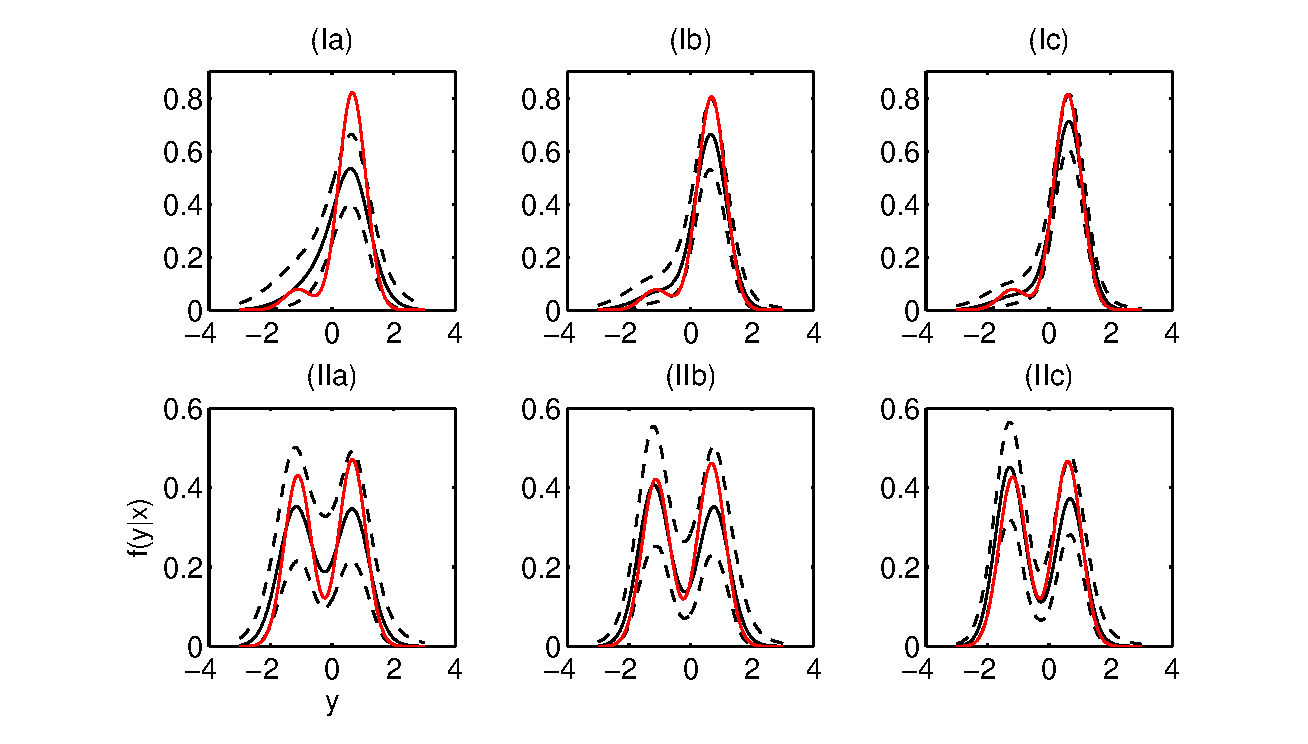
\includegraphics[width=120mm]{../figs/ch3_density.eps}
 \vskip -15pt 
% 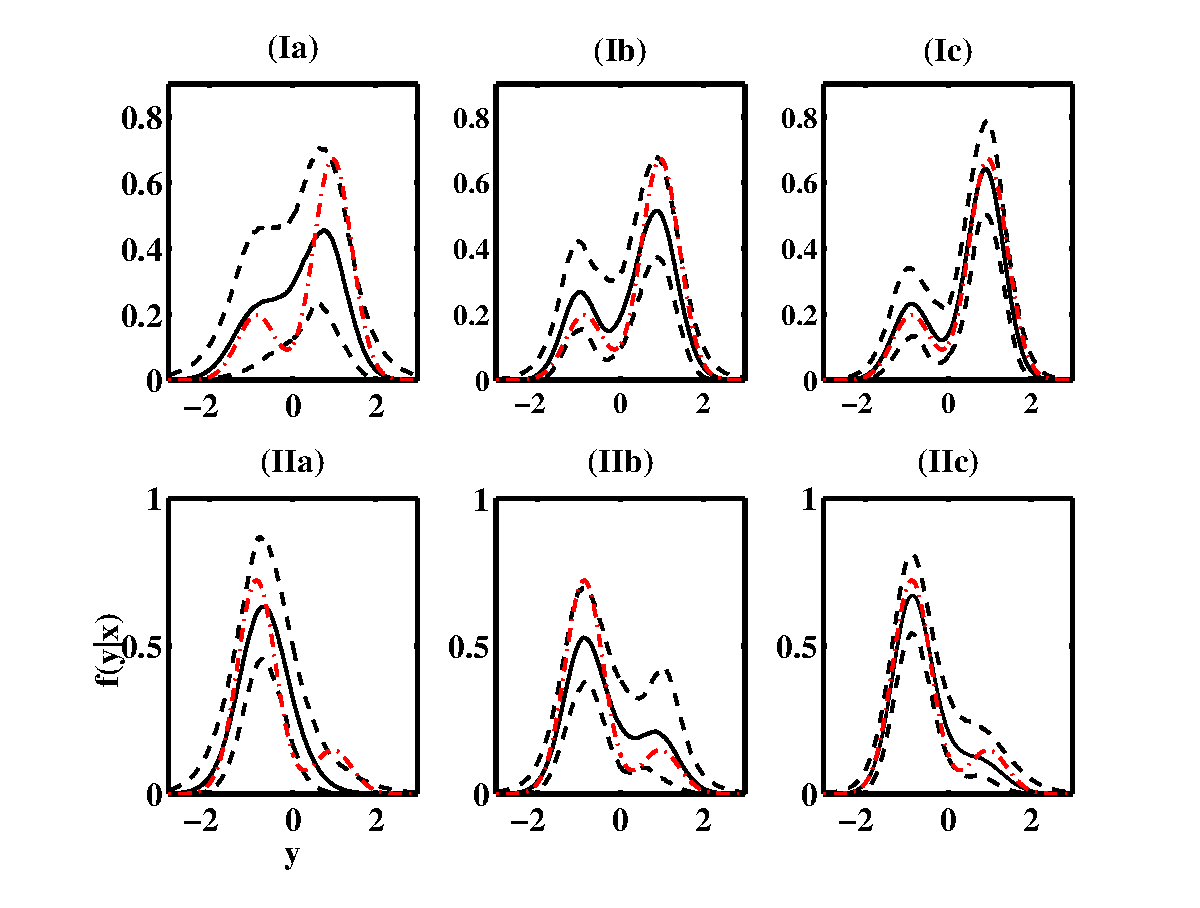
\includegraphics[width=90mm,height=80mm]{densityestimate.eps}
\caption{Illustrative example: Plot of true (red line) and estimated density ($50$th percentile: solid line, $2.5$th and $97.5$th percentiles: dashed lines) for two data points $(I, II)$ considering different training set size (a:100, b:150, c:200). } \label{plotDensity}
\end{figure}




\subsection{Quantitative Comparisons} 


Figure \ref{fig:boxplots}(I) shows boxplots of $r_{mse}^{\mc{A}}$ as $p$ increases. Clearly, our method outperforms the competitors in terms of mean squared errors. Furthermore, as shown in figure \ref{fig:linear}(II), our approach can scale substantially better than competitors to huge dimensions of the predictor space. 




\begin{figure}[h!]
\centering
 \vskip -0pt 
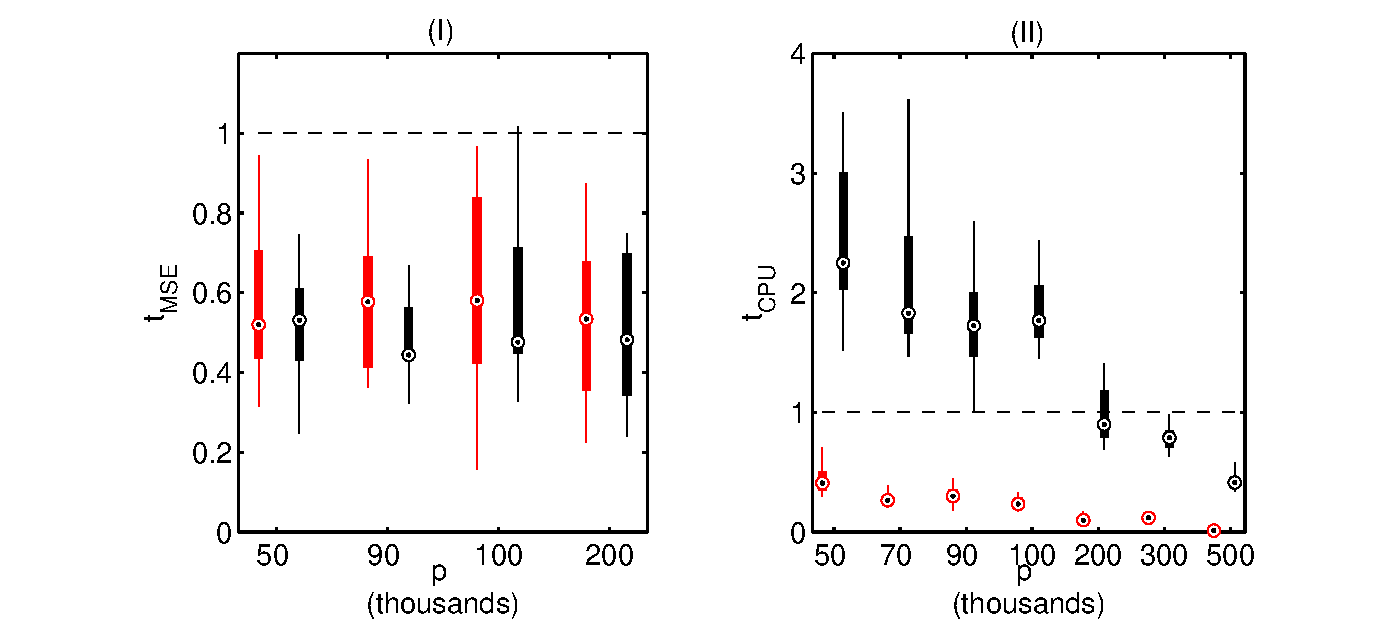
\includegraphics[width=.6\linewidth]{../figs/experiment1.eps} 
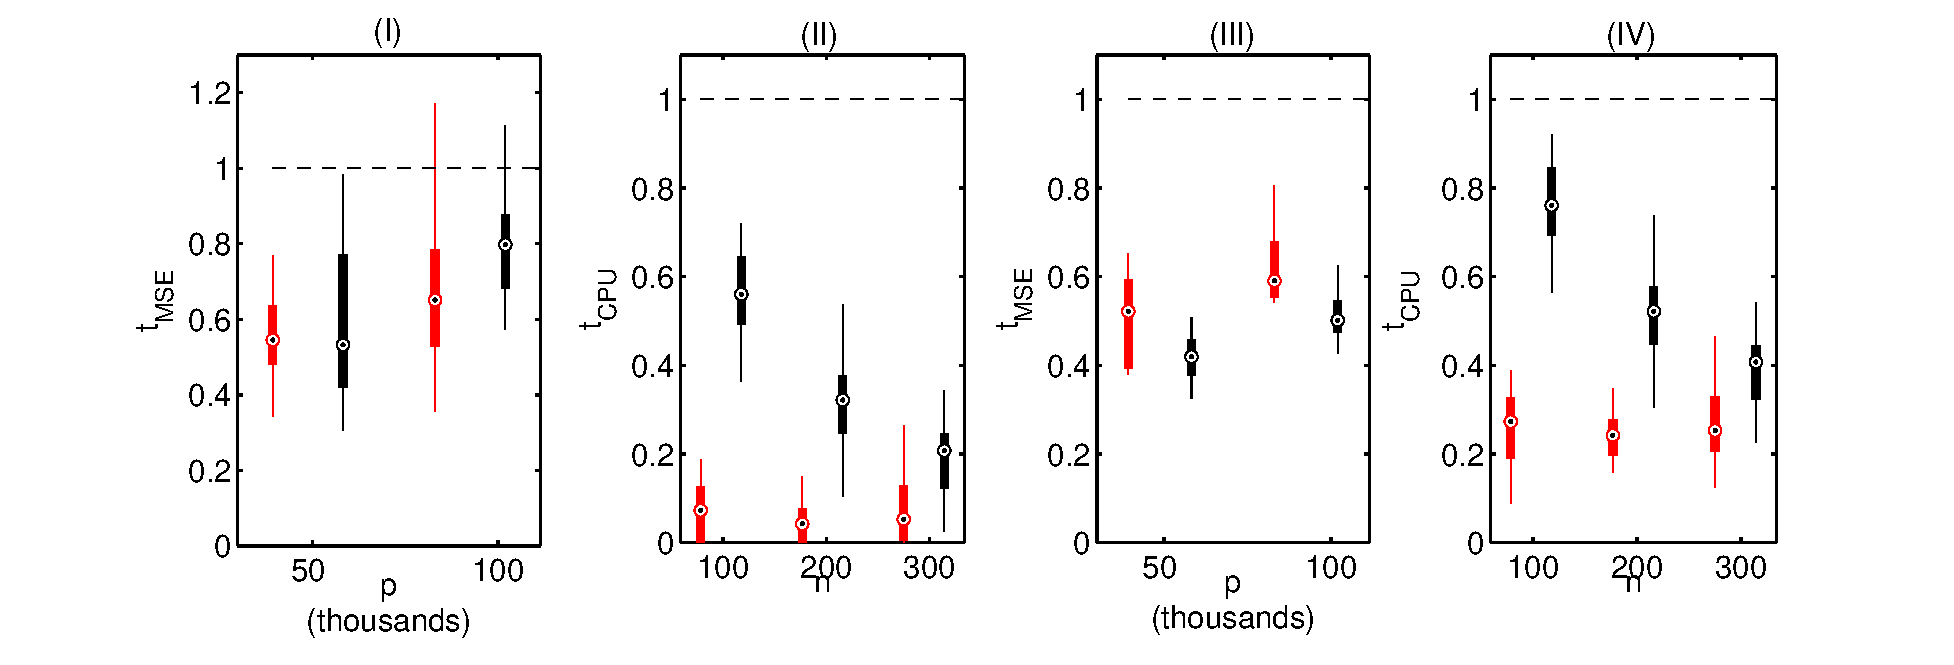
\includegraphics[width=0.8\linewidth]{../figs/nonlinear.eps} 

 \vskip -10pt 

% 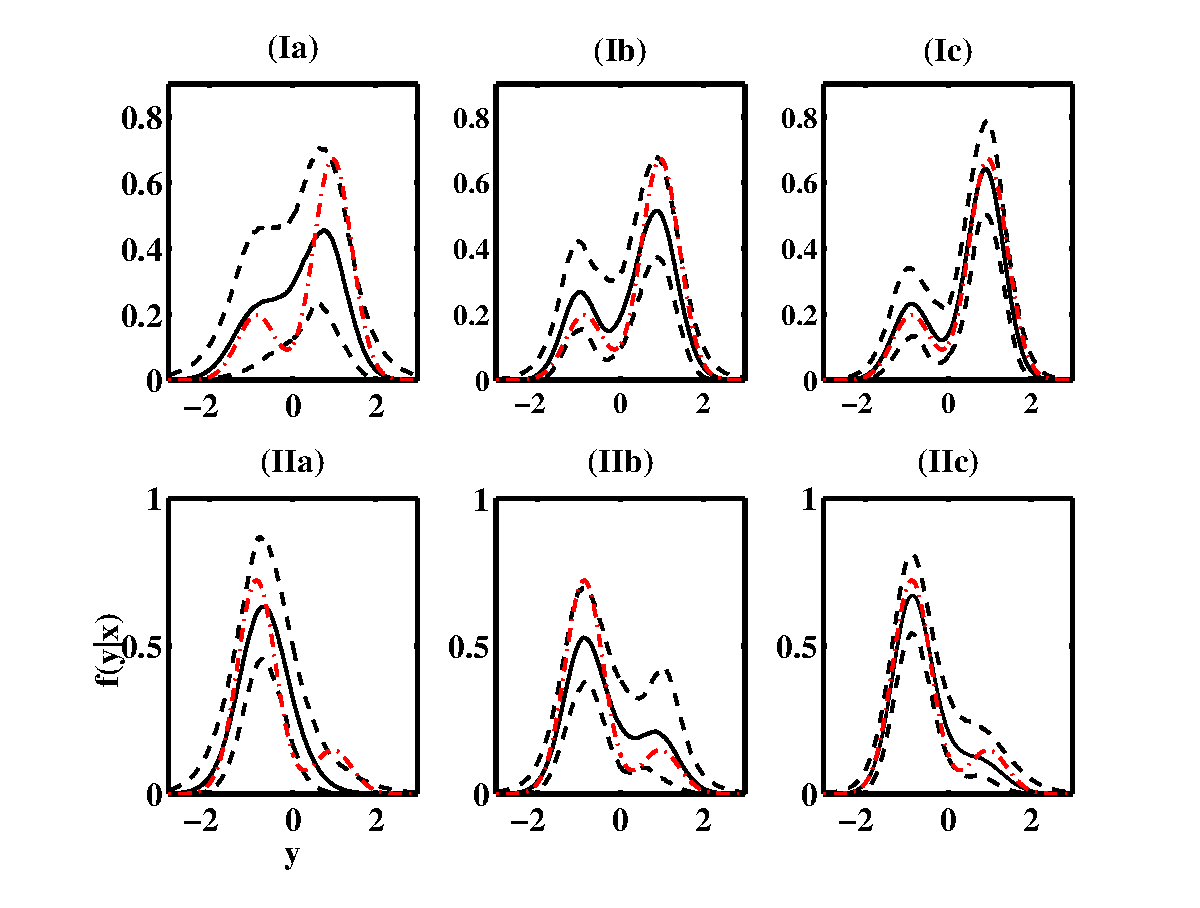
\includegraphics[width=90mm,height=80mm]{densityestimate.eps}
\caption{Numerical results for various simulation scenarios.  Top (bottom) plots depict the relative mean-squared error (CPU time in seconds) of our approach, MSB, versus CART (red) and Lasso (black).  The three simulation scenarios are: \eqref{eq:linear} (left), \eqref{eq:MFA} (middle) and \eqref{eq:swiss} (right). MSB outperforms both CART and Lasso in all three scenarios regardless of ambient dimension ($r_{mse}^{\mc{A}}< 1$ for all $p$).  MSB compute time is relatively constant as $n$ or $p$ increase, whereas Lassso's compute time increases, thus, as $n$ or $p$ increase, MSB CPU time becomes less than Lasso's.  MSB was always significantly faster than CART, regardless of $n$ or $p$.} 
% (I) Boxplots of $ r^{\mc{A}}_{mse}$ as $p$ increases. (II) Boxplot of $r^{\mc{A}}_{cpu}$ with $\mc{A}$=CART (red) and $\mc{A}$=Lasso (black) under data drawn from the factor model in \ref{eq:factor}.
% Boxplots of $r^{\mc{A}}_{mse}$ under data drawn from MFA (I) and swissroll (III) and boxplots of $r^{\mc{A}}_{cpu}$ for a fixed $p=300,000$ and different $n$ under data drawn from MFA (II) and swissroll (IV) with $\mc{A}$=CART (red) and $\mc{A}$=Lasso (black).} 
\label{fig:boxplots}
\end{figure}

 
Figure \ref{MFA:plot}(I) and  \ref{MFA:plot}(III)  show boxplots of $r_{mse}^{\mc{A}}$.  Again our model is associated to better predictive performance compared to CART and Lasso. To show how the performance of our model varies for different sample sizes,  we sampled datasets involving different number of observations. In practice, the dimension of the predictor space was considered fixed, i.e. $p=300,000$ and ratios $r^{\mc{A}}_{cpu}$ were computed considering sample sizes $n \in \{100,200,300 \}$. Figure \ref{MFA:plot}(II) and  \ref{MFA:plot}(IV) show that our model can scale better than competitors to high dimensions and its performance improves as the sample size increases. 



% \begin{figure}[h!]
% \centering
%  \vskip 0pt 
% 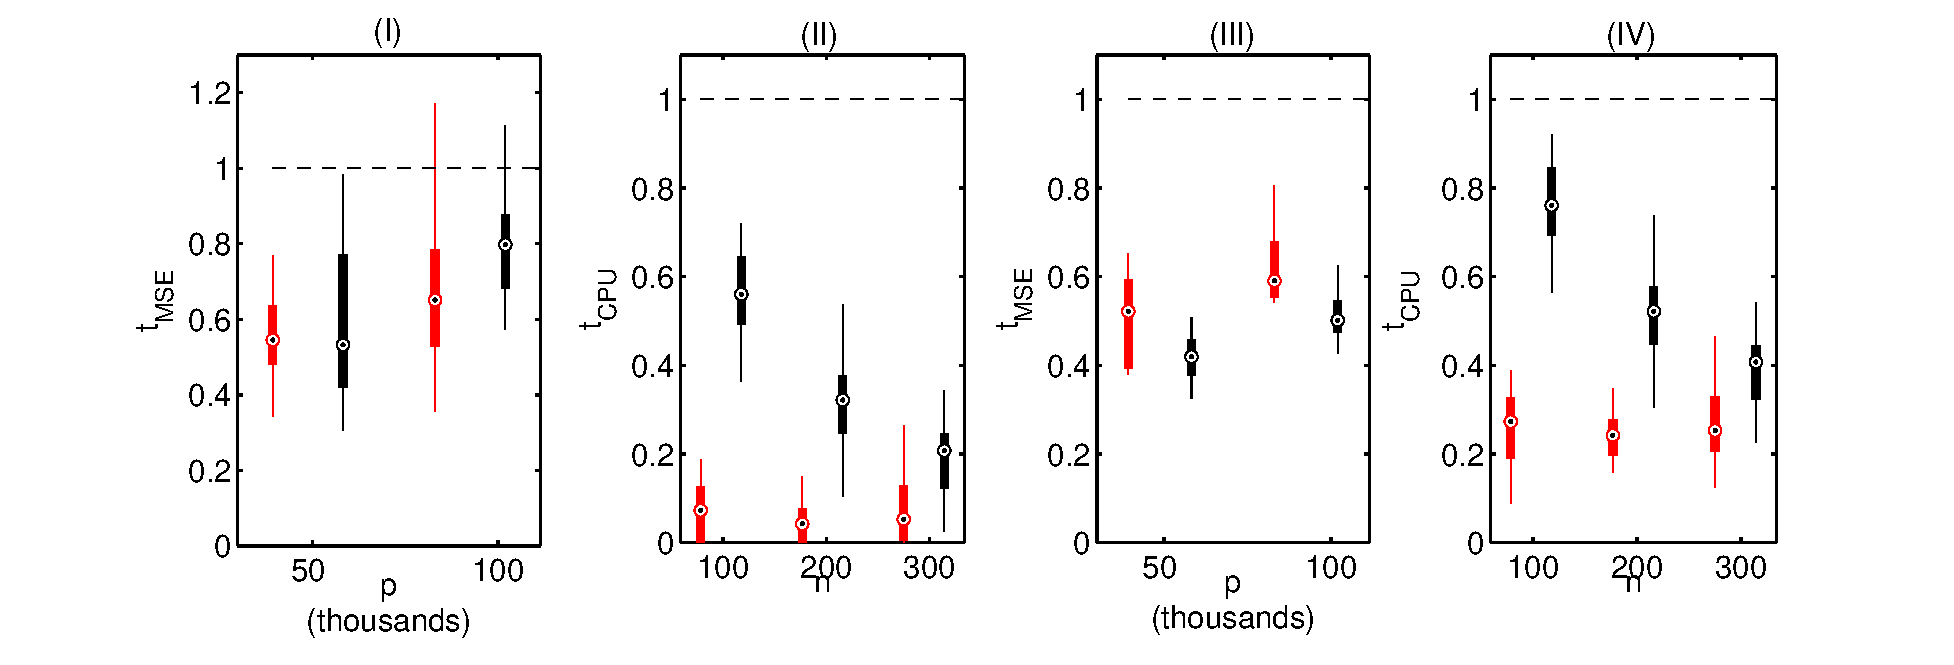
\includegraphics[width=1.0\linewidth]{../figs/nonlinear.eps} 
%  \vskip -10pt 
% \caption{Boxplots of $r^{\mc{A}}_{mse}$ under data drawn from MFA (I) and swissroll (III) and boxplots of $r^{\mc{A}}_{cpu}$ for a fixed $p=300,000$ and different $n$ under data drawn from MFA (II) and swissroll (IV) with $\mc{A}$=CART (red) and $\mc{A}$=Lasso (black).} \label{MFA:plot} % \label{swiss:plot}
% \end{figure}


\subsection{Neuroscience Applications} \label{sub:real}

We assessed the predictive performance of the proposed method on two very different neuroimaging datasets. First, we consider a structural connectome dataset collected at the Mind Research Network.  Data were collected as described in Jung et al. \cite{Jung2010}. For the analysis, all variables were normalized by subtracting the mean and dividing by the standard deviation. The same prior specification and Gibbs sampler as in \S 3 was  utilized. 

In the first experiment we investigated the extent to which we could predict creative (as measured via the Composite Creativity Index \cite{Arden2010}).   For each subject, we estimate a $70$ vertex undirected weighted brain-graph using the Magnetic Resonance Connectome Automated Pipeline \cite{MRCAP11} from diffusion tensor imaging data \cite{Mori2006}. Because our graphs are undirected and lack self-loops, we have a total of $\binom{70}{2}=2,415$ potential weighted edges. The vector of covariates consists in the natural logarithm of the total number of connections between all pairs of cortical regions, i.e. $p=2,415$. 

The second dataset comes from a resting-state functional magnetic resonance experiment as part of the Autism Brain Imaging Data Exchange \cite{Autism}.  We selected the Yale Child Study Center for analysis.  Each brain-image was processed using the Configurable Pipepline for Analysis of Connectomes \cite{cpac}. For each subject we computed a measure of normalized power at each voxel called fALFF \cite{Zou2008}.  To ensure the existence of nonlinear signal relating these predictors, we let $y_i$ correspond to an estimate of overall head motion in the scanner, called mean framewise displacement (FD) computed as described in Power et al. \cite{power}. 

Table \ref{real} shows mean and variance squared error based on leave-one-out predictions. Variable $r_{T}$ is the amount of time necessary to obtain predictions for all subjects, while variables $r_M$ and $r_V$ are respectively the mean and the standard deviation of amount of time necessary to obtain one point predictions. For the first data example, we compared our approach (multiscale stick-breaking; MSB) to CART, Lasso and random forests. 
Table \ref{real} shows that MSB outperforms all the competitors in terms of mean square error; this is in addition to yielding an estimate of the entire conditional density for each $y_i$.  It is also significantly faster that random forests, the next closest competitor, and faster than Lasso.  For this relatively low-dimensional example, CART is reasonably fast.   For the second data application, given the huge dimensionality of the predictor space, we were unable to get either CART or random forest to run to completion, yielding memory faults on our workstation (Intel Core i7-2600K Quad-Core Processor memory 8192 MB).  We thus only compare performance to Lasso.  As in the previous example, MSB outperforms Lasso in terms of predictive accuracy measured via mean-squared error, and significantly outperforms Lasso in terms of computational time.  
 % and the poor scalability of CART and random forest, the comparison was made only with Lasso. As shown in table \ref{real}, our approach is more efficient and accurate than Lasso in predicting the response variable. 
%Figure \ref{fig:real} shows the plot of CPU time used to predict each one of the $56$ subjects involved in the experiment. The time needed to compute quantities utilized in all subject predictions was divided equally across subjects. Clearly, our approach is able to improve the computational time by up to five orders of magnitude. 


\begin{table}[t]
\caption{Real Data: Mean and standard deviations of squared error under multiscale stick-breaking (MSB), CART, Lasso and random forest (RF).  Variable $r_{T}$ is the amount of time necessary to obtain predictions for all subjects, while variables $r_M$ and $r_V$ are respectively the mean and the standard deviation of amount of time necessary to obtain one point predictions.}\label{real}
\vskip 0.15in
\begin{center}
\begin{small}
\begin{sc}
\begin{tabular}{llcccccccc}
\hline
data &$n$&$p$ &model&mse&$r_{T}$ & $r_{M}$ & $r_{V}$\\
\hline
(1)&108&2,415&msb &$0.56$ & $100$ & $1.1$& $0.02$\\
 &&& CART & $1.10$ & $87$ & $0.9$ &$0.01$\\
&&& Lasso & $0.63$  & $50$ & $0.40$ & $0.10$\\
&&& rf & $0.57$ &  $7,817$ & $78.2$ & $0.59$\\
\\
  (2)&56&$10e+05$&msb &$0.76$ & $690$ & $20.98$& $2.31$\\
 &&& Lasso & $1.02$  & $5,836$ & $96.18$ & $9.66$\\
\hline
\end{tabular}
\end{sc}
\end{small}
\end{center}
\vskip -0.1in
\end{table}


% \nocite{langley00}

\dd{we gotta remove about 10 references to make our reference list fit} 

\bibliographystyle{unsrt} 
\bibliography{nipsMSB} 


\end{document}
